% -%-%-%-%-%-%-%-%-%-%-%-%-%-%-%-%-%-%-%-%-%-%-%-%-%
% MDI224 % 
% Data:12/12/2011                                 %
% Paris,France                                    % 
% Groupe:                                         %
% - Tiago Chedraoui Silva                   % 
% - Anthony CLERBOUT
% -%-%-%-%-%-%-%-%-%-%-%-%-%-%-%-%-%-%-%-%-%-%-%-%-%

\documentclass[a4paper,11pt]{article}

\usepackage[francais,listings,algo]{tcs}

% Cover %
\def \ttprofname{Roland BADEAU} % teachers name
\def \ttabrv{MDI224} % abbreviation of names class
\def \ttabrvxt{} % period
\def \mytitle{Interpolation par splines cubiques} % Big title
\def \mysubtitle{ Travaux Pratique 1 - Deuxième semestre de 2011} % subtitle
\def \ttauthi{Anthony CLERBOUT} % author's name
\def \ttxti{Casier: 234} % Extra text right side of name
\def \ttauthii{Tiago CHEDRAUOI SILVA} % author's name
\def \ttxtii{Casier: 214 } % Extra text right side of name
\def \ttdate{Décembre 15, 2011} % date

\begin{document}
\titleTMB 
\newpage
\tableofcontents
\listoffigures
\newpage

\section{Résolution du système linéaire}

\subsection{Méthode de Jacobi}
\subsubsection{Implémentation}

Pour voir la méthode de Jacobi, on a fait le code suivant:

\begin{multicols}{2}
  \lstinputlisting[title=\textbf{Méthode de Jacobi}]{../jacobi.m}
\end{multicols}

\newpage

Pour  voir le  convergence  de la  méthode de  Jacobi,  on a  pris, pour  chaque
itération, chaque valeur de x
calculé jusqu'au moment que méthode arrête. Après, on a fait la comparaison de
chaque x avec le valeur optimal (xex) en prenant le log de la différence:

\subsubsection{Convergence}
\begin{figure}[h!]
  \begin{centering}
    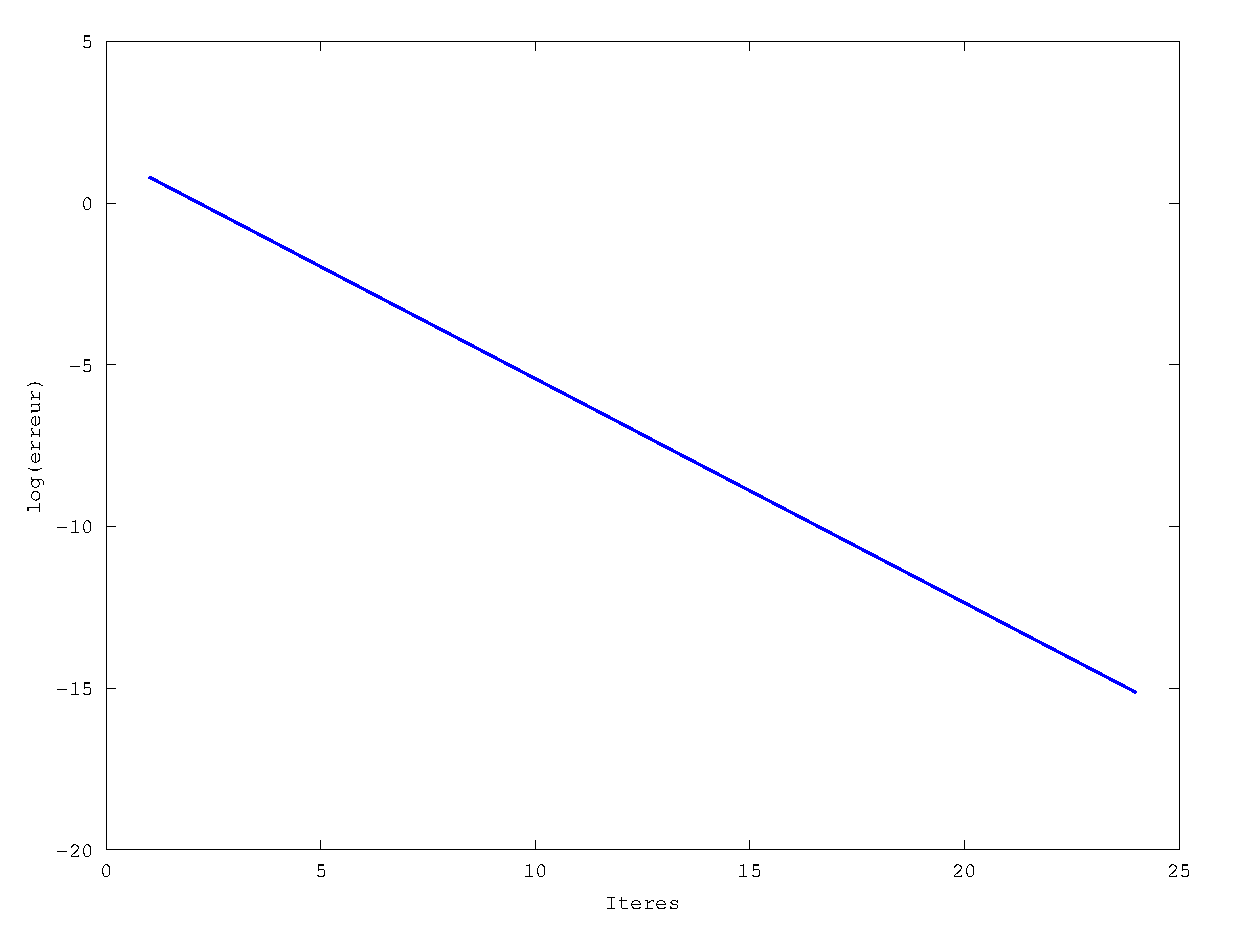
\includegraphics[scale=0.5]{../jacobi_graph}
    \label{rspro2}
    \par\end{centering}
  \caption{Convergence de la méthode de Jacobi}
  \label{fig:jacobi-conv}
\end{figure}

En utilisant la fonction polyfit, nous avons trouvé le polynome: 
$p(x)= -0.693147 x + 1.497866  $


\subsection{Méthode de relaxation}
Pour voir la méthode SOR (relaxation), on a fait le code suivant:

\subsubsection{Implémentation}
\begin{multicols}{2}
  \lstinputlisting[title=\textbf{Méthode de Jacobi}]{../relax.m}
\end{multicols}

Pour  voir le  convergence  de la  méthode SOR,  on a  pris, pour  chaque
itération, chaque valeur de x
calculé jusqu'au moment que méthode arrête ( pour w=1.0). Après, on a fait la comparaison de
chaque x avec le valeur optimal (xex) en prenant le log de la différence:


\subsubsection{Convergence}
\begin{figure}[h!]
  \begin{centering}
    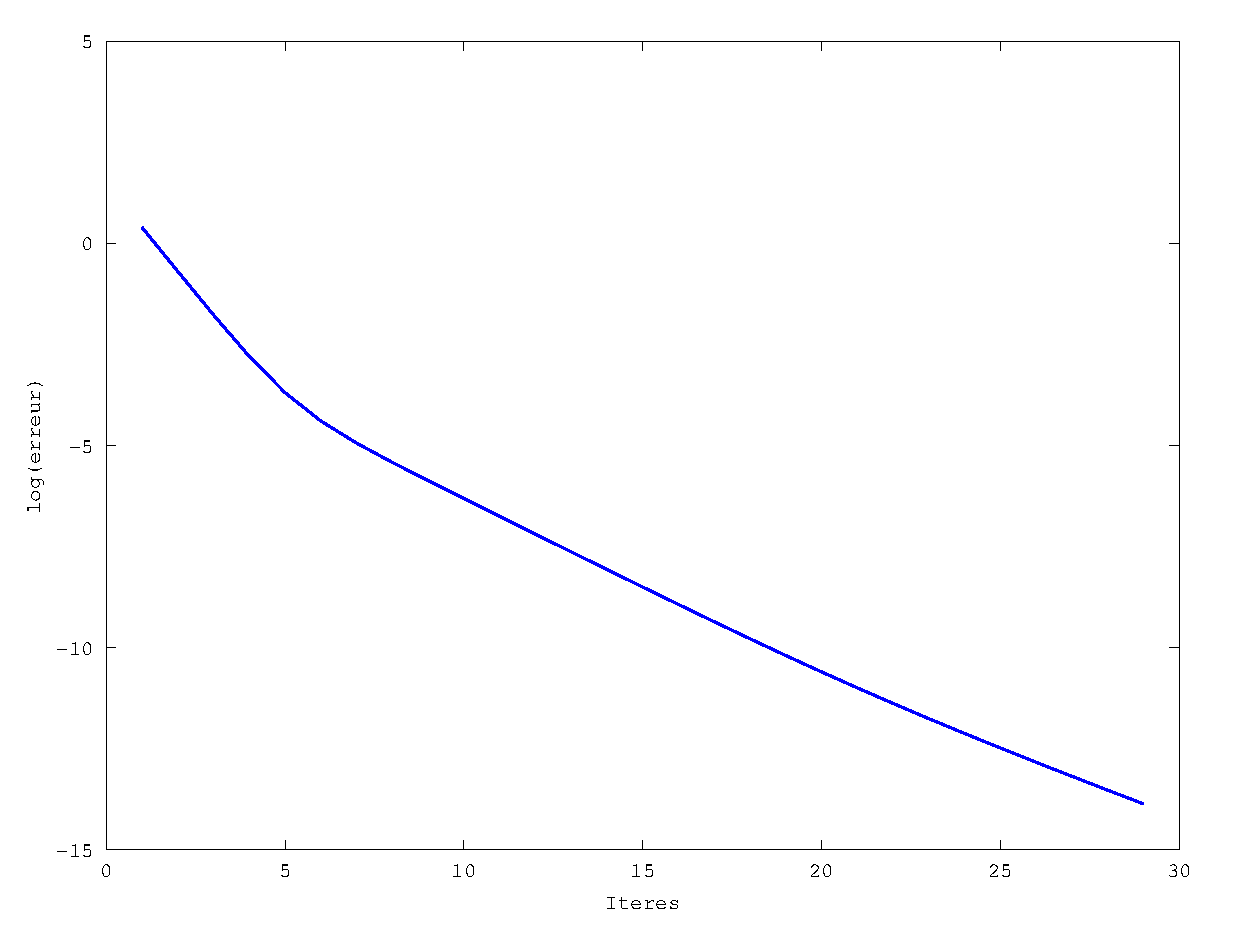
\includegraphics[scale=0.5]{../relaxation_graph}
    \label{rspro2}
    \par\end{centering}
  \caption{Convergence de la méthode de Relaxation pour w=1.0}
  \label{fig:jacobi-conv}
\end{figure}




Pour voir le  taux, il existe deux méthodes, le premier,  il utilise les erreurs
et la fonction polyfit de matlab. Le deuxième il calcule le rayon spectral de la
matrice  $R_w$. Ainsi,  on change  les valeurs  de $w$  de manière  a  trouve le
meieller taux de convergence. Les graphes  pour les deux approches sont vue dans
les graphes en 3 et 4 bas.
On a trouve un $w_{optmal}\approx 1.1$ 

\begin{figure}[h!]
  \begin{centering}
    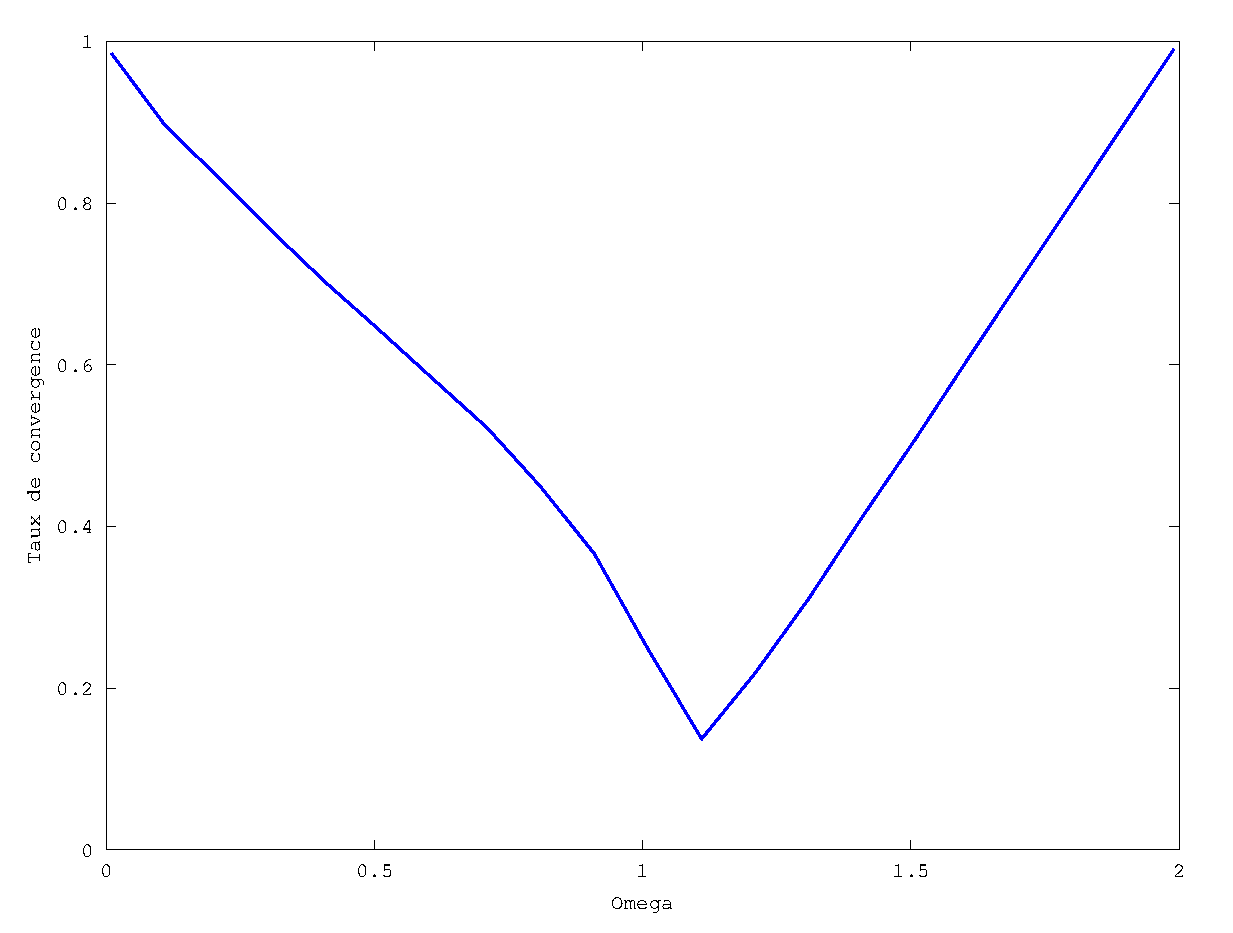
\includegraphics[scale=0.5]{../relaxation_conv2}
    \label{rspro2}
    \par\end{centering}
  \caption{Approche 1:Taux de convergence en fonction du paramètre de relaxation w}
  \label{fig:jacobi-conv}
\end{figure}

\begin{figure}[h!]
  \begin{centering}
    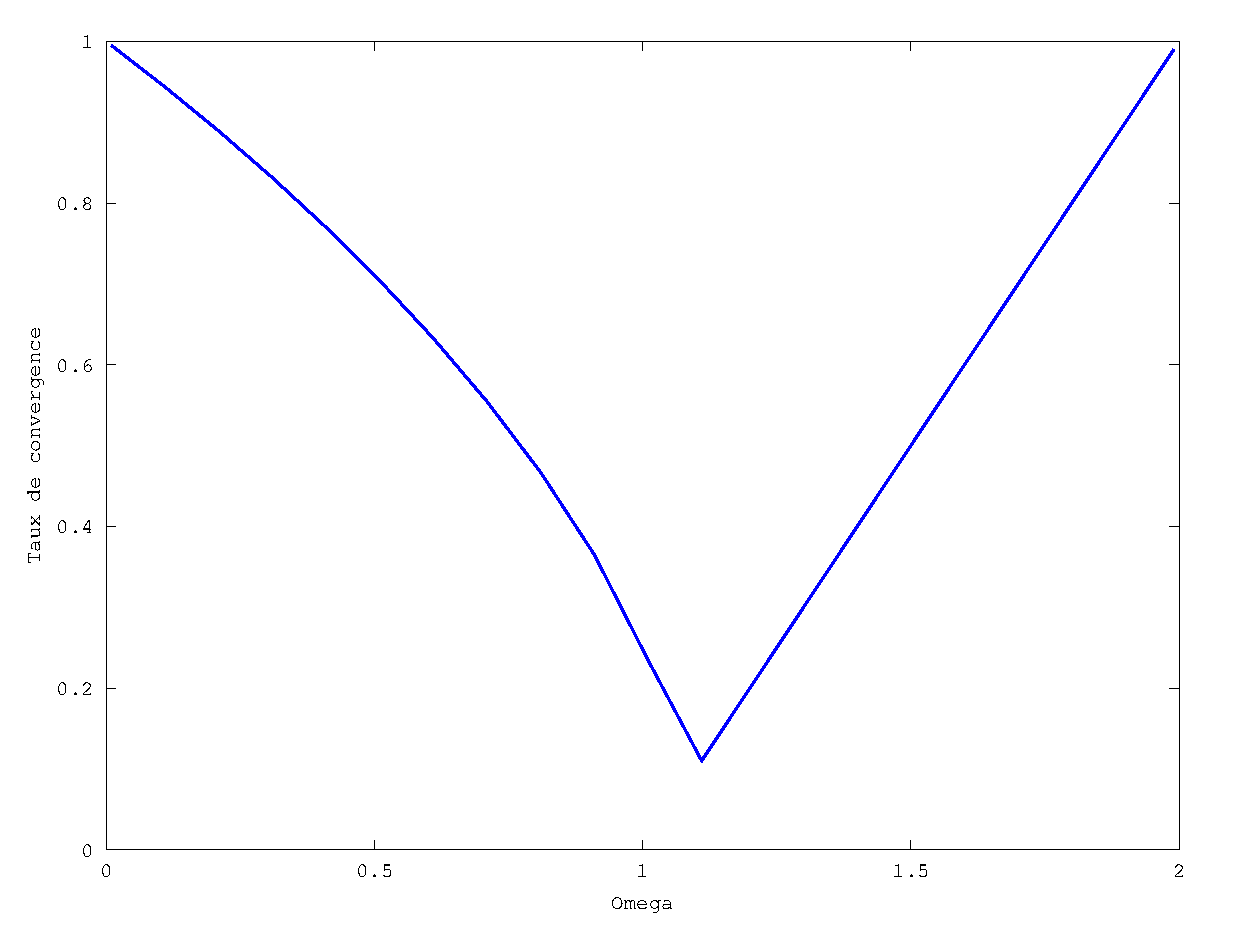
\includegraphics[scale=0.5]{../relaxation_conv_rho}
    \label{rspro2}
    \par\end{centering}
  \caption{Approche 2: Calcule du rayon spectral de la matrice $R_w$}
  \label{fig:jacobi-conv}
\end{figure}

%\begin{equation}
%  \omega = \frac{2}{1+\sqrt{1- \rho(J)^2}}
%\end{equation}

%\begin{equation}
%  \frac{d\omega}{d\rho} =\frac{2\,\rho}{\sqrt{1-{\rho}^{2}}\,{\left( \sqrt{1-{\rho}^{2}}+1\right) }^{2}}
%\end{equation}

%Pour le valeur  minimum ou maximum la dérivée doit être  0, donc $\rho(J)=0$, en
%utilisant la équation 1 on a $\omega=1$;

\newpage
\subsection{Méthode de Cholesky}
\subsubsection{Implémentation}

La fonction suivante était fournit par le problème. 
\begin{multicols}{2}
  \lstinputlisting[title=\textbf{Méthode de Jacobi}]{../cholesky.m}
\end{multicols}

Pour le même exemple précedent, on a trouve:

\begin{table}[h!]
  \begin{center}
    \begin{tabular}{|c|c|}
      \hline 
      p & x \\
      \hline 
      \hline 
      4 & [ 1.00000;1.00000;1.00000;1.00000;1.00000]\\
      3 & [ 1.00000;1.00000;1.00000;1.00000;1.00000]\\
      2 & [ 1.00000;1.00000;1.00000;1.00000;1.00000]\\
      1 & [ 1.00000;1.00000;1.00000;1.00000;1.00000]\\
      \hline 
    \end{tabular}
  \end{center}
  \caption{Vérification function Cholesky}
\end{table}

\subsubsection{Complexité}

\begin{table}[h!]
  \begin{center}
    \begin{tabular}{|c|c|c|c|c|c|c|}
      \hline 
      N & 50 & 100 & 150 & 200 & 250 & 300 \\
      \hline 
      \hline 
      Cholesky $(p=1)$ & 0.011554       &  0.023093 & 0.036068
      & 0.047571 & 0.061026 & 0.074059 \\
      Jacobi &   0.0026100
      &    0.0031020
      &   0.0041549
      &   0.0048039
      &  0.0078550
      &  0.0097679        \\
      Relaxation $(w = 1.1)$
      &  0.0020840
      &  0.0025171
      & 0.0036389 
      & 0.0065949
      & 0.0083960
      & 0.018082\\
      \hline 
    \end{tabular}
  \end{center}
  \caption{Comparaison de temps entre les trois méthodes pour un système tridiagonal}
\end{table}

En général le méthode Relaxation (SOR) est la méthode plus rapide pour un
système tridiagonal, parce que il  fait moins itération que Jacobi, peut-être le
code n'est pas optimal c'est pour cela que le temps pour N grand est grand.

\section{Application}
\subsection{Calcul d'une spline d'interpolation}
\begin{multicols}{2}
  \lstinputlisting[title=\textbf{Méthode spline cubique}]{../sinterp.m}
\end{multicols}

\subsection{Évaluation d'une fonction spline cubique}


\begin{multicols}{2}
  \lstinputlisting[title=\textbf{Méthode spline cubique}]{../speval.m}
\end{multicols}

\subsection{Application}

En utilisant les  fonctions mis en œuvre avant, on a utilisé les fonctions sinus
et exponentielle pour vérifier le spline cubique. Les graphes suivantes sont les valeurs interpolées par le
spline cubique et l'erreur de cette interpolation si on comparé aux valeurs de la fonction réel.

 Une observation, pour les graphes des erreurs,  les points  en 0  sont le  points utilisées pour trouver  les valeurs
pendand l'interpolation, c'est-à-dire, sont le point en commun entre le fonction
réel et l'interpolée, donc il n'existe pas d'erreur parce que c'est le même valeur.
D'autre remarque est que plus le valeur de la fonction est grand, plus est l'erreur.

\begin{figure}[h!]
  \begin{centering}
    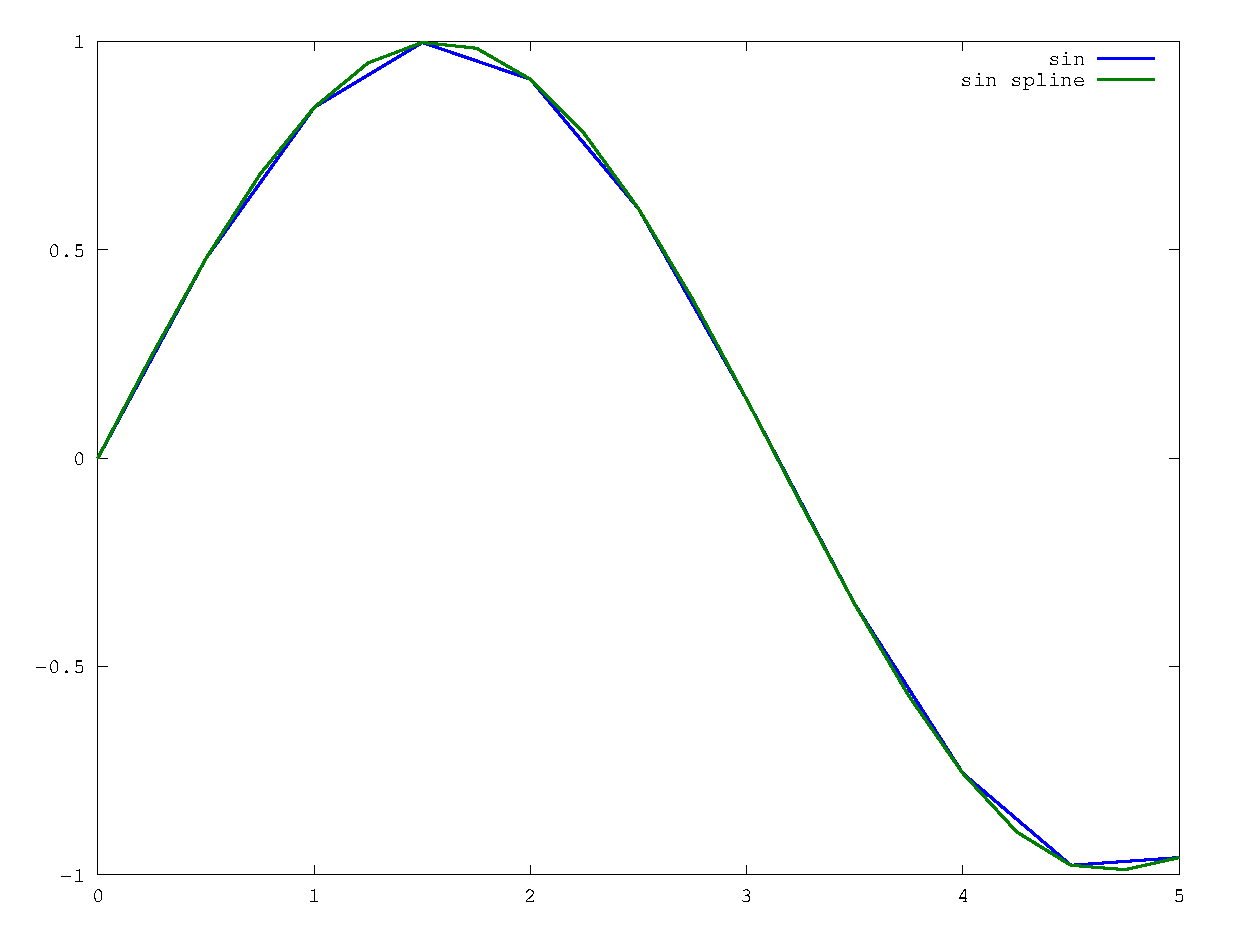
\includegraphics[scale=0.5]{../sinus_2}
    \label{rspro2}
    \par\end{centering}
  \caption{Spline Cubique - fonction sinus pas original 0.5, pas spline 0.25}
  \label{fig:jacobi-conv}
\end{figure}

\begin{figure}[h!]
  \begin{centering}
    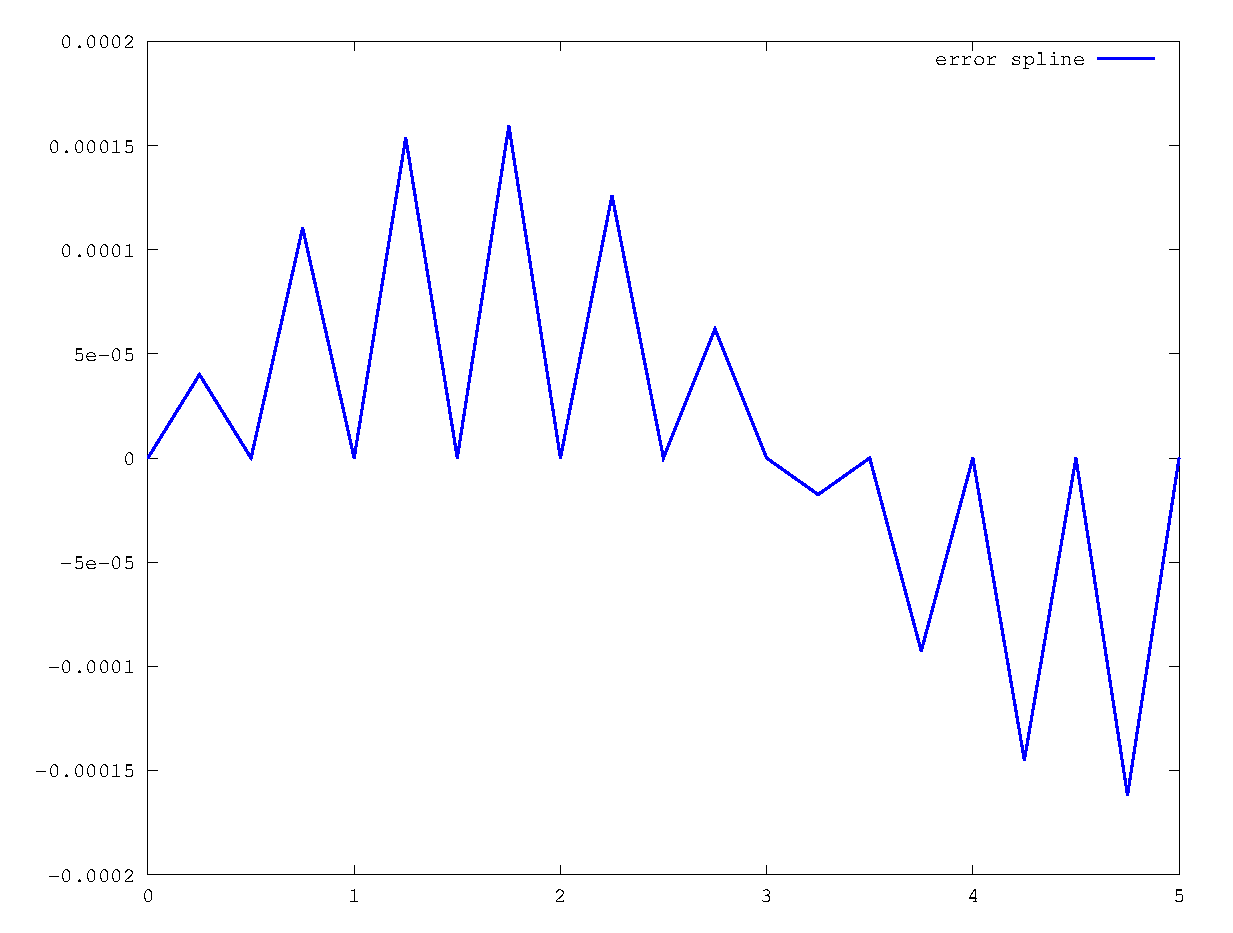
\includegraphics[scale=0.5]{../sinus_2_error}
    \label{rspro2}
    \par\end{centering}
  \caption{Error Spline Cubique - fonction sinus pas original 0.5, pas spline 0.25}
  \label{fig:jacobi-conv}
\end{figure}


\begin{figure}[h!]
  \begin{centering}
    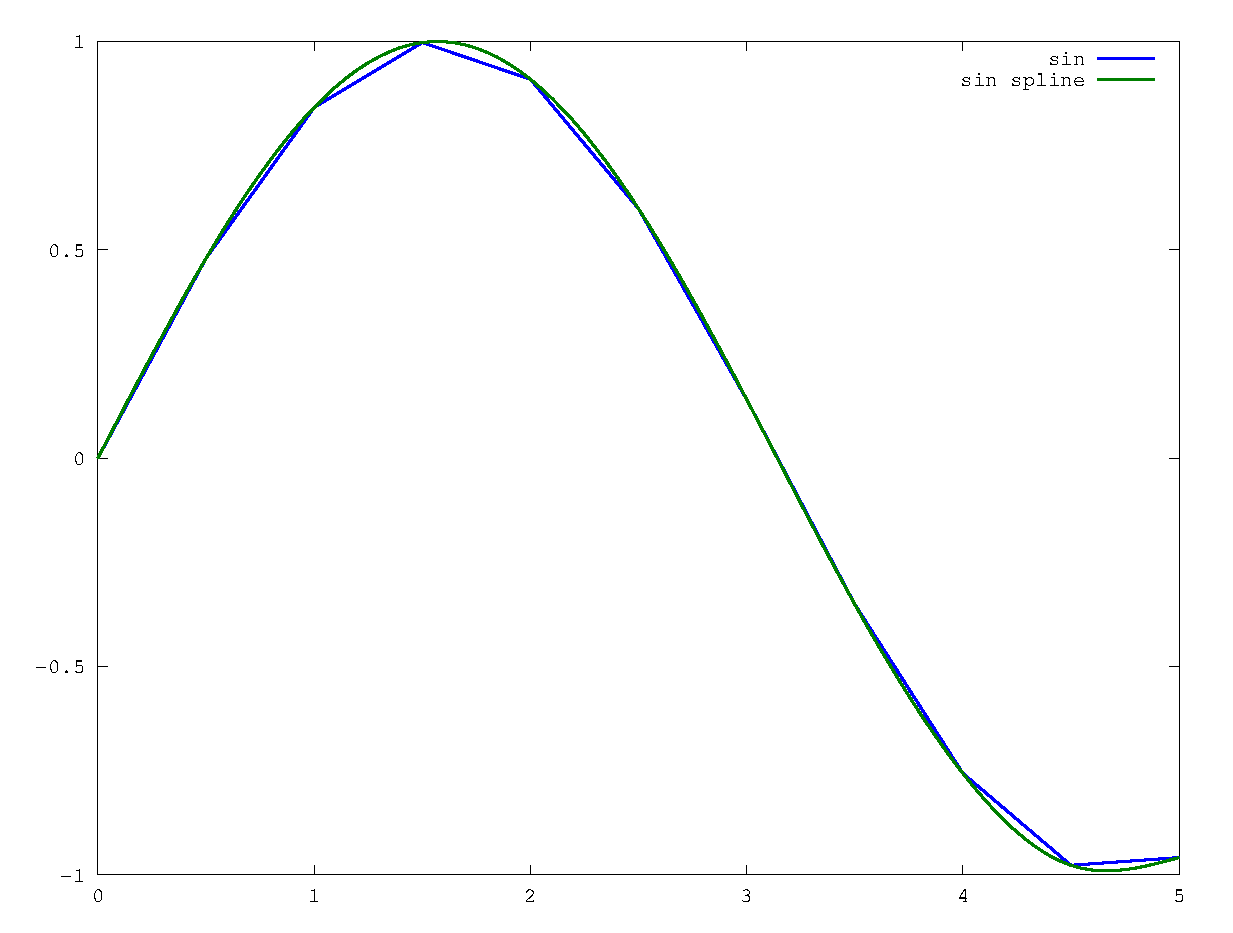
\includegraphics[scale=0.5]{../sinus_5}
    \label{rspro2}
    \par\end{centering}
  \caption{Spline Cubique - fonction sinus pas original 0.5, pas spline 0.1}
  \label{fig:jacobi-conv}
\end{figure}


\begin{figure}[h!]
  \begin{centering}
    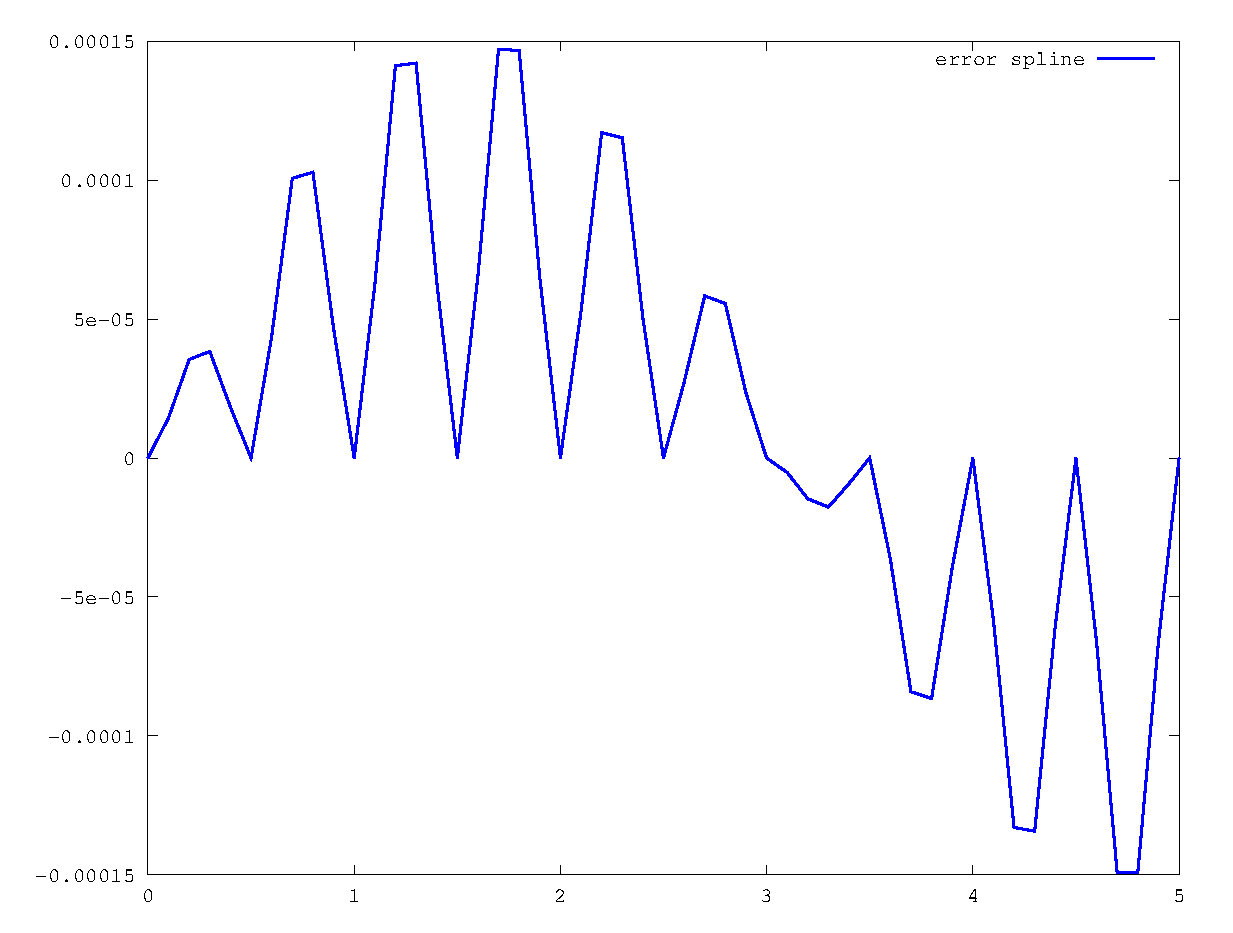
\includegraphics[scale=0.5]{../sinus_5_error}
    \label{rspro2}
    \par\end{centering}
  \caption{Error Spline Cubique - fonction sinus pas original 0.5, pas spline 0.25}
  \label{fig:jacobi-conv}
\end{figure}

\begin{figure}[h!]
  \begin{centering}
    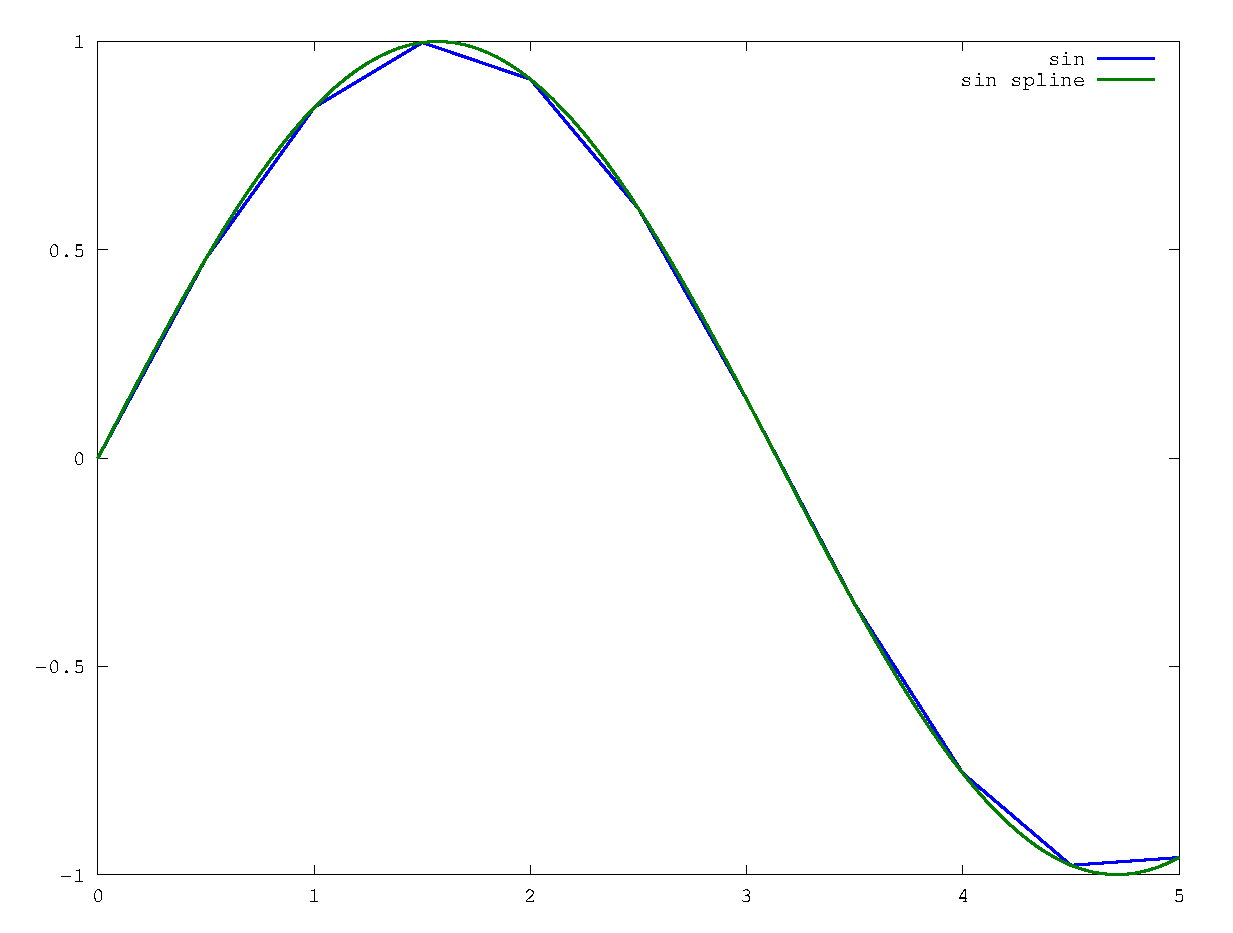
\includegraphics[scale=0.5]{../sinus_10}
    \label{rspro2}
    \par\end{centering}
  \caption{Spline Cubique - fonction sinus pas original 0.5, pas spline 0.05}
  \label{fig:jacobi-conv}
\end{figure}


\begin{figure}[h!]
  \begin{centering}
    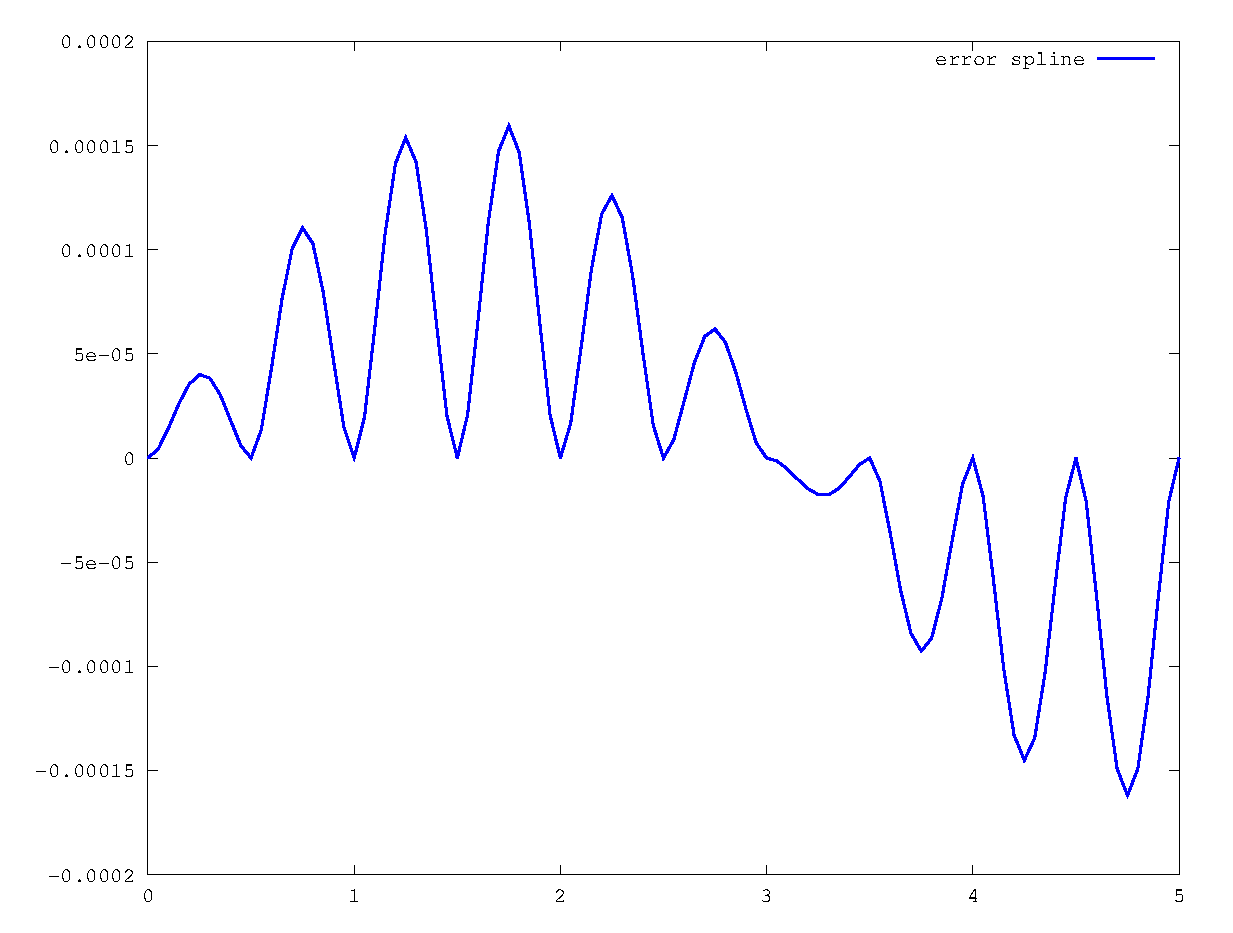
\includegraphics[scale=0.5]{../sinus_10_error}
    \label{rspro2}
    \par\end{centering}
  \caption{Error Spline Cubique - fonction sinus pas original 0.5, pas spline 0.25}
  \label{fig:jacobi-conv}
\end{figure}

\begin{figure}[h!]
  \begin{centering}
    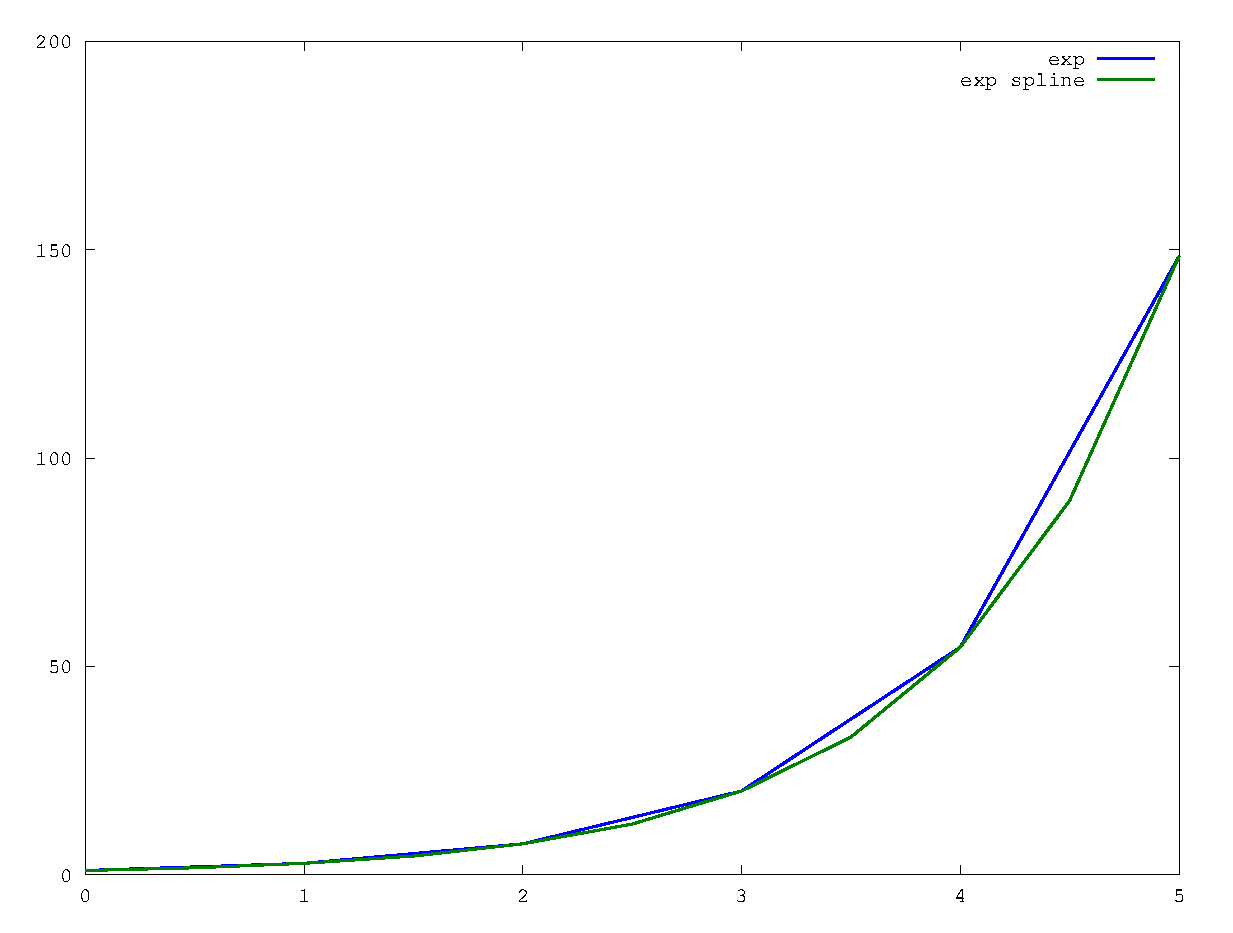
\includegraphics[scale=0.5]{../exp_2}
    \label{rspro2}
    \par\end{centering}
  \caption{Spline Cubique - fonction exp pas original 1, pas spline 0.5}
  \label{fig:jacobi-conv}
\end{figure}


\begin{figure}[h!]
  \begin{centering}
    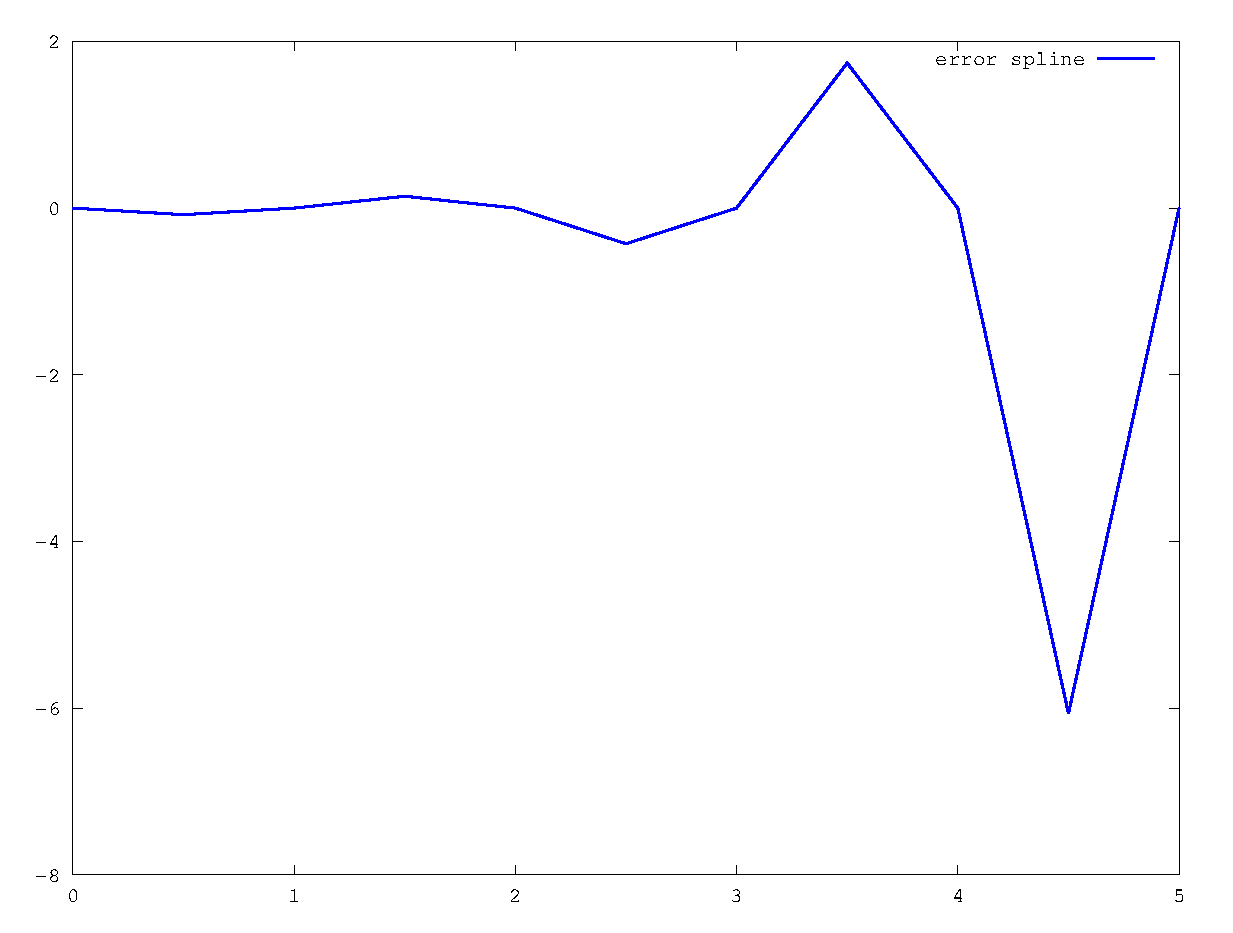
\includegraphics[scale=0.5]{../exp_2_error}
    \label{rspro2}
    \par\end{centering}
  \caption{Error Spline Cubique - fonction exp pas original 1, pas spline 0.5}
  \label{fig:jacobi-conv}
\end{figure}

\begin{figure}[h!]
  \begin{centering}
    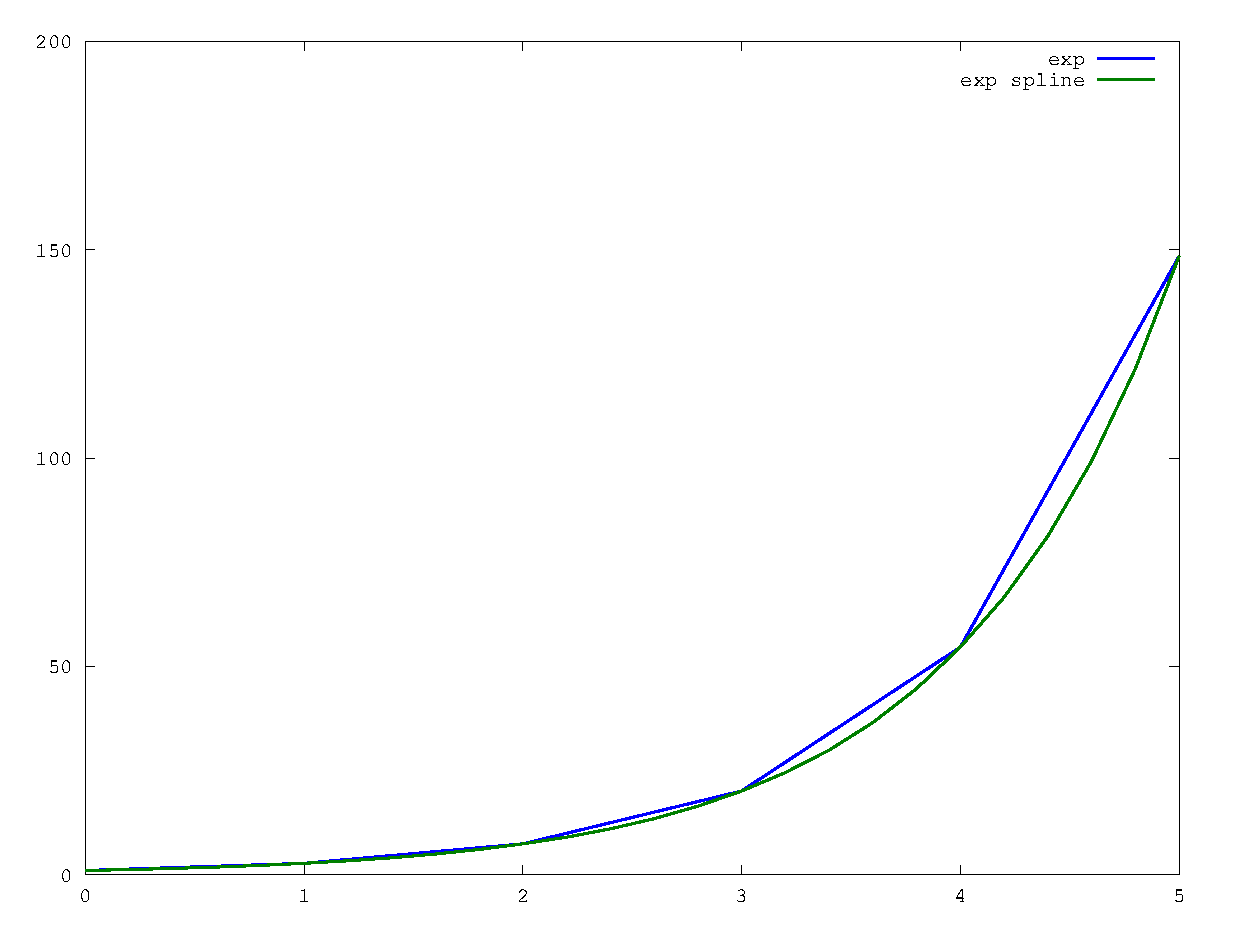
\includegraphics[scale=0.5]{../exp_5}
    \label{rspro2}
    \par\end{centering}
  \caption{Spline Cubique - fonction exp pas original 1, pas spline 0.02}
  \label{fig:jacobi-conv}
\end{figure}

\begin{figure}[h!]
  \begin{centering}
    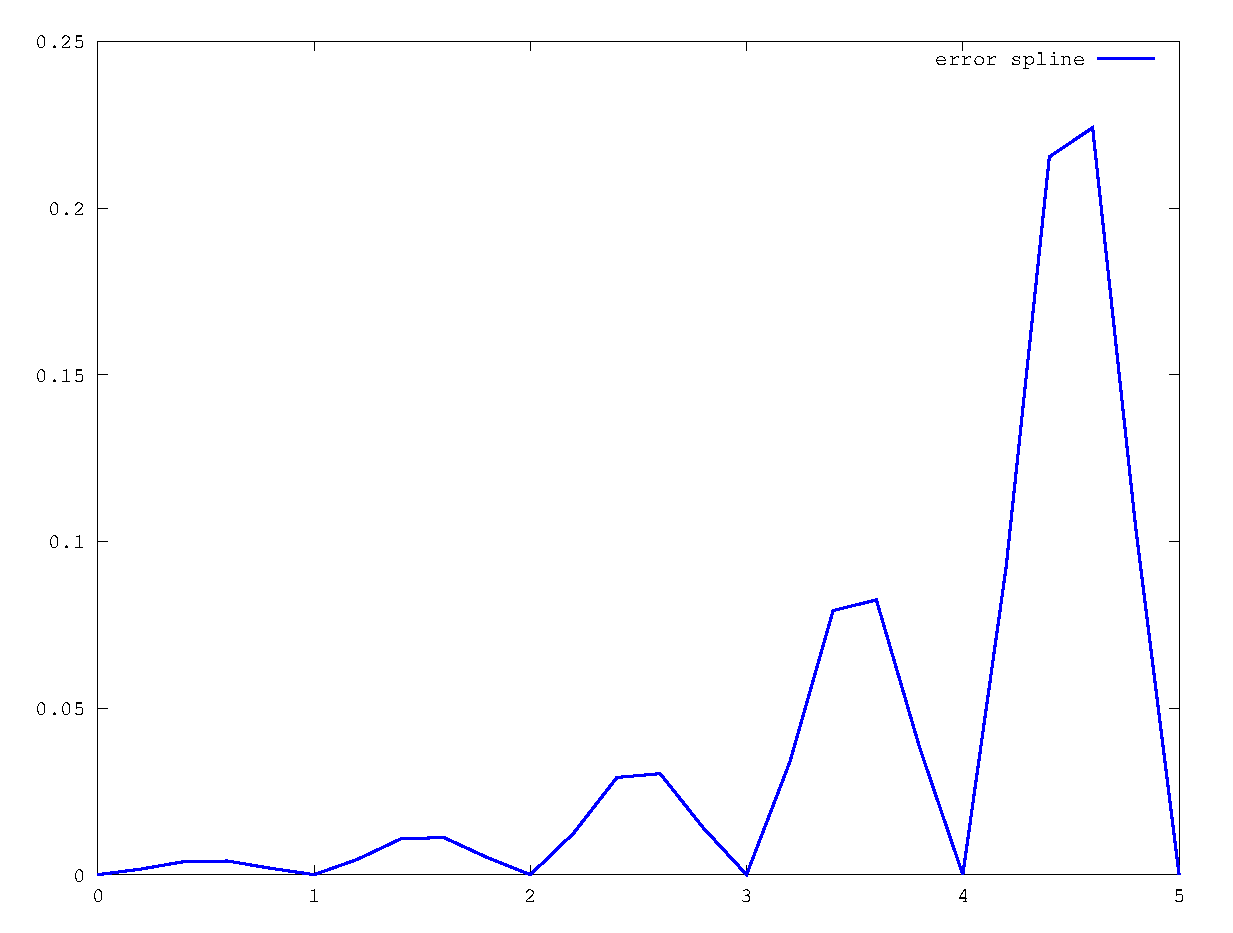
\includegraphics[scale=0.5]{../exp_5_error}
    \label{rspro2}
    \par\end{centering}
  \caption{Error Spline Cubique - fonction exp pas original 1, pas spline 0.5}
  \label{fig:jacobi-conv}
\end{figure}


\begin{figure}[h!]
  \begin{centering}
    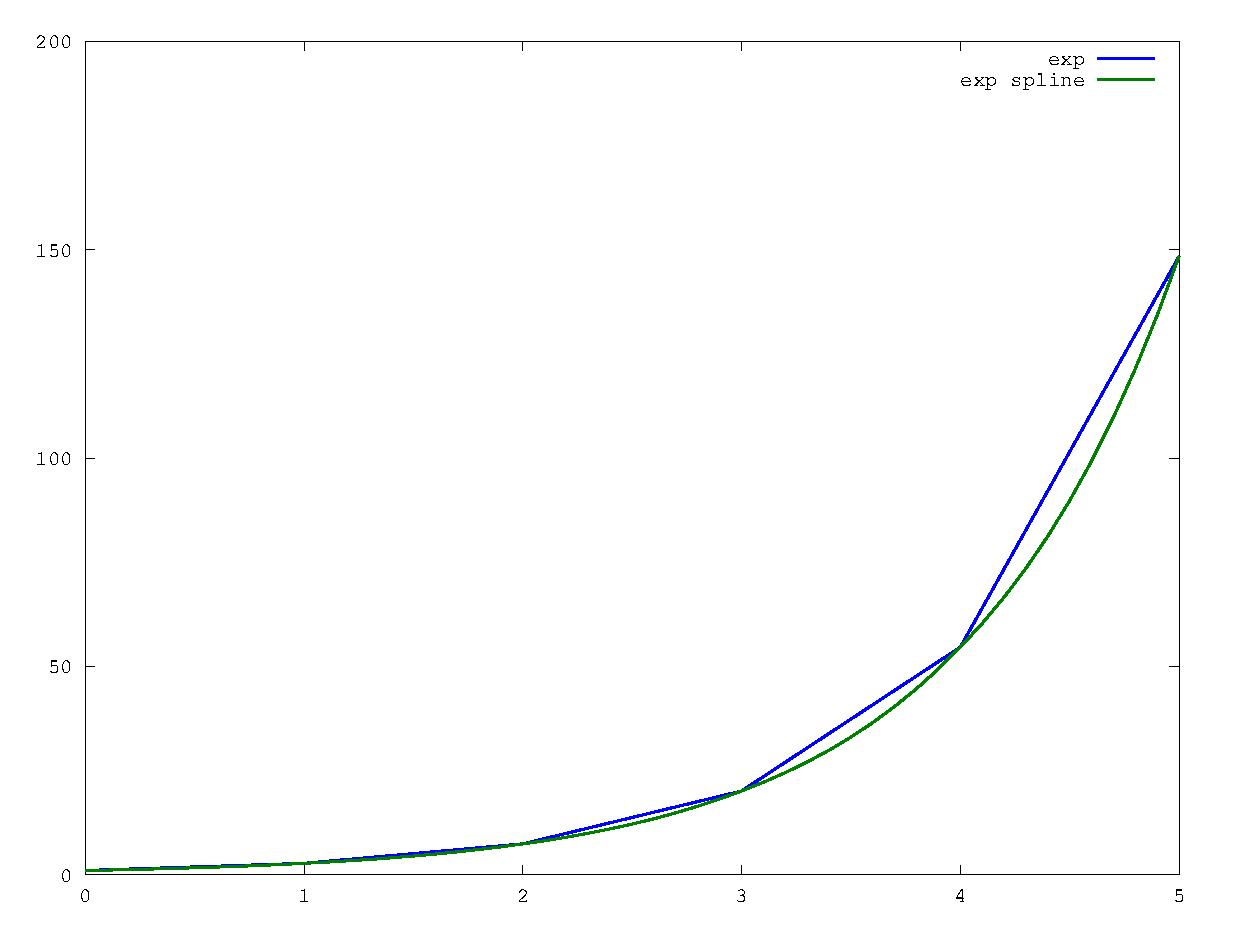
\includegraphics[scale=0.5]{../exp_10}
    \label{rspro2}
    \par\end{centering}
  \caption{Spline Cubique - fonction exp pas original 1, pas spline 0.1}
  \label{fig:jacobi-conv}
\end{figure}

\begin{figure}[h!]
  \begin{centering}
    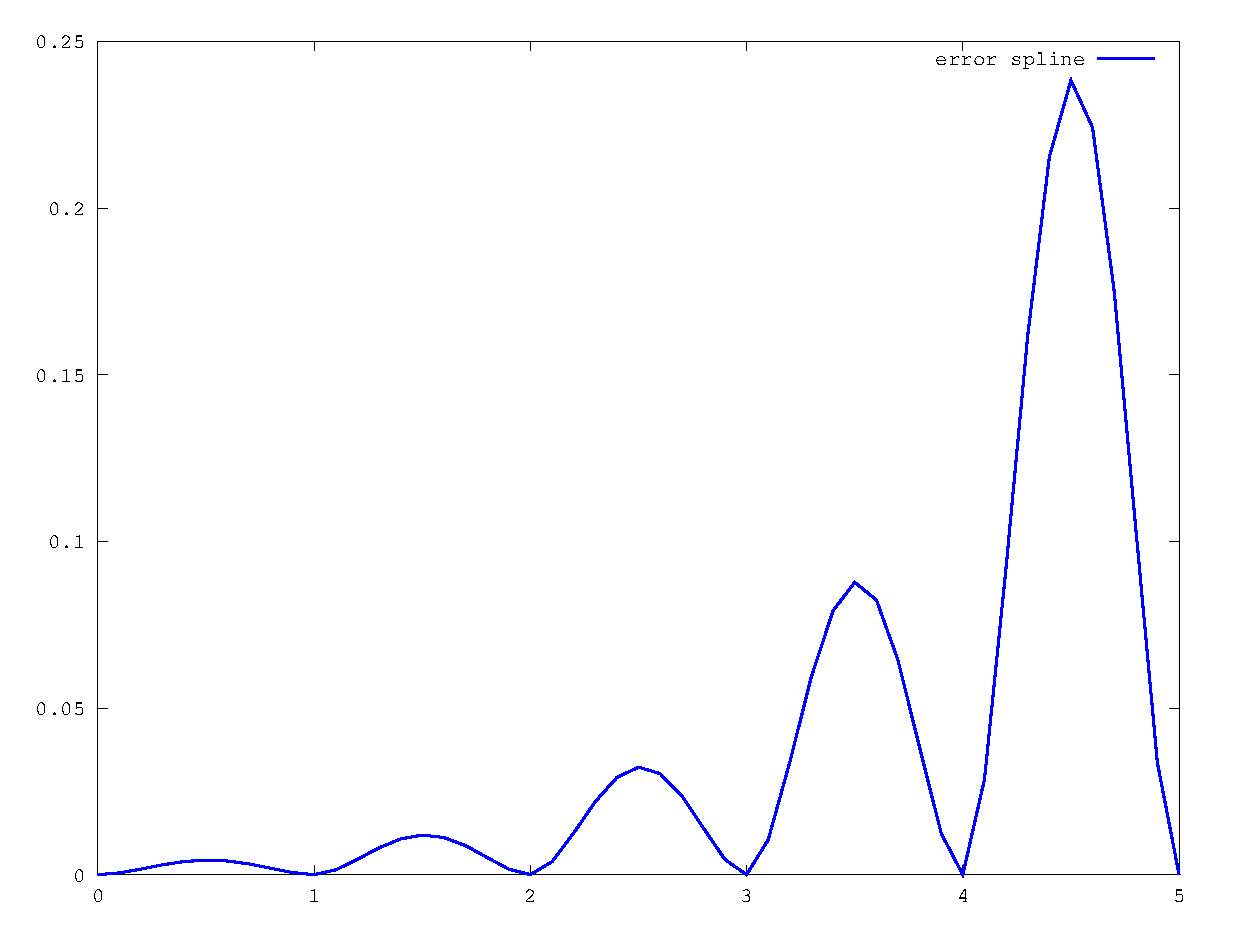
\includegraphics[scale=0.5]{../exp_10_error}
    \label{rspro2}
    \par\end{centering}
  \caption{Error Spline Cubique - fonction exp pas original 1, pas spline 0.5}
  \label{fig:jacobi-conv}
\end{figure}


\begin{figure}[h!]
  \begin{centering}
    \subfigure[Interpolation]{
      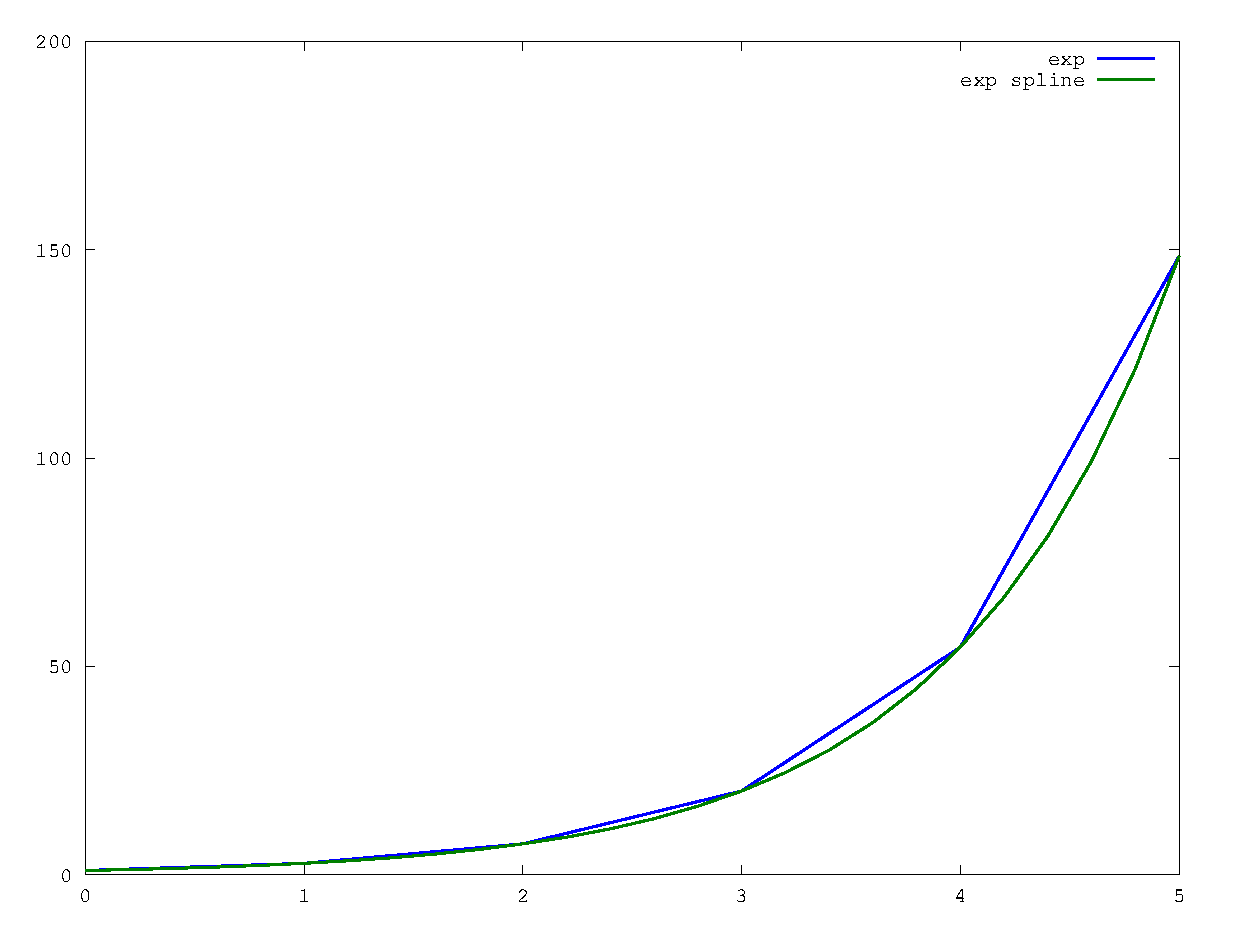
\includegraphics[scale=0.35]{../exp_5}    }
    \subfigure[Erreur interpolation.]{
      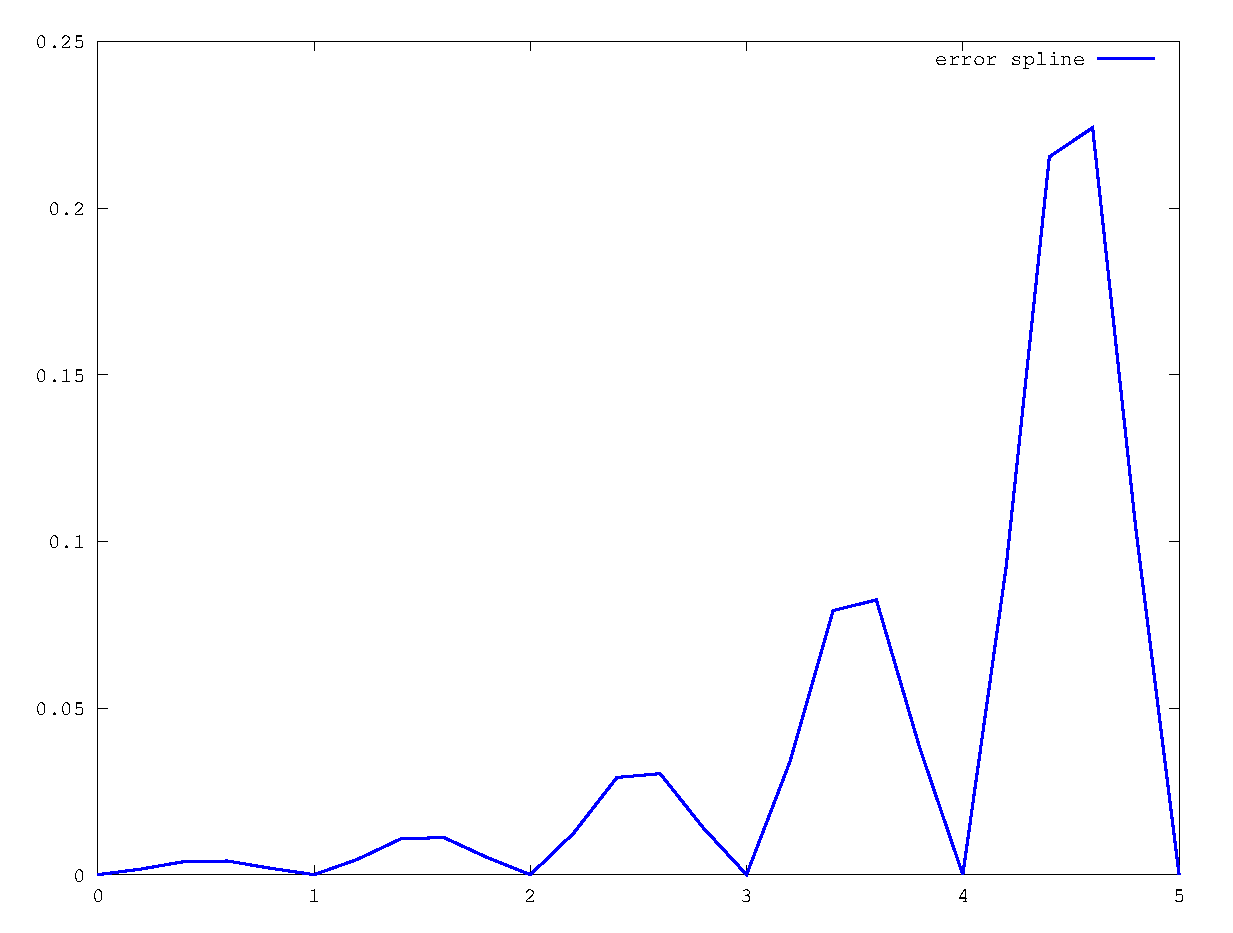
\includegraphics[scale=0.35]{../exp_5_error}
    }
    \par\end{centering}
  \caption{Fonction exp pas original 1, pas spline 0.1}
  \label{rspro}
\end{figure}


\begin{figure}[h!]
  \begin{centering}
    \subfigure[Interpolation]{
      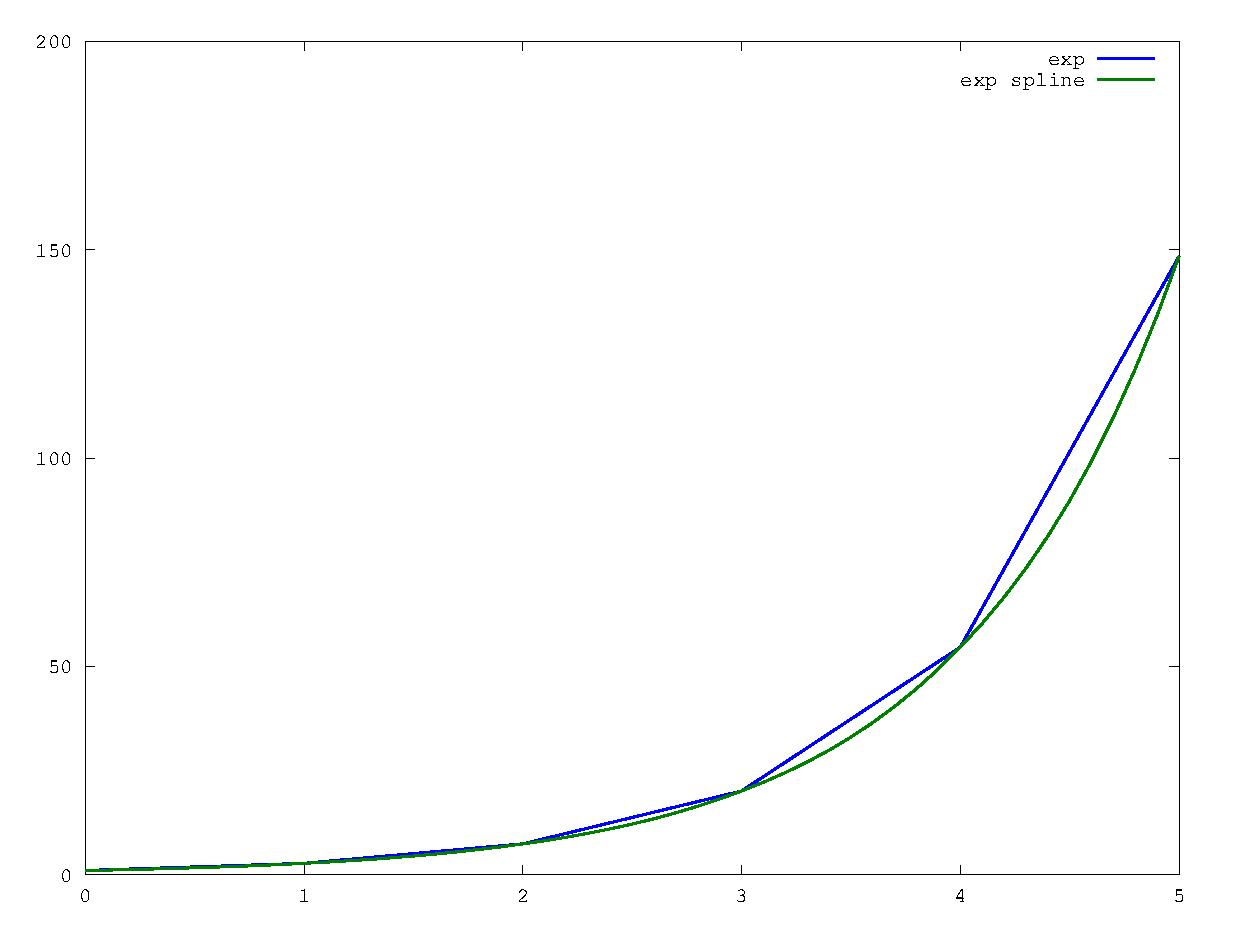
\includegraphics[scale=0.35]{../exp_10}    }
    \subfigure[Erreur interpolation.]{
      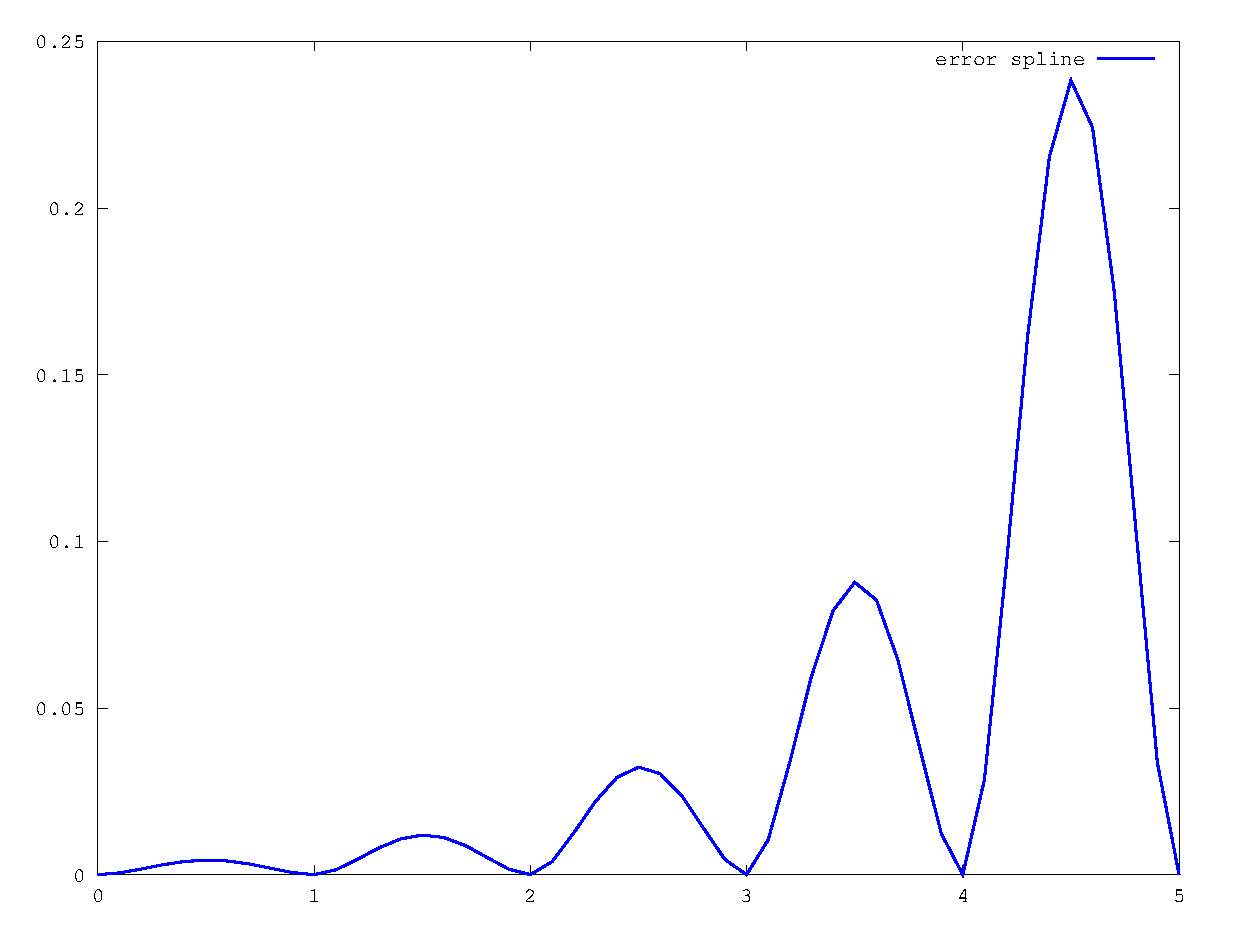
\includegraphics[scale=0.35]{../exp_10_error}
    }
    \par\end{centering}
  \caption{Fonction exp pas original 1, pas spline 0.5}
  \label{rspro}
\end{figure}

\end{document}

